\documentclass[12pt]{article}
\usepackage[spanish]{babel}
\usepackage{geometry}
\geometry{a4paper, margin=1in}
\usepackage{graphicx}
\usepackage{xcolor}
\usepackage{titlesec}
\usepackage{parskip}
\usepackage{multicol}
\usepackage{cite}

\definecolor{highlight}{RGB}{255, 255, 0}

\titleformat{\section}{\normalfont\Large\bfseries}{\thesection}{1em}{}
\titleformat{\subsection}{\normalfont\large\bfseries}{\thesubsection}{1em}{}

\begin{document}

% Logos
\begin{minipage}{0.45\textwidth}
    
\includegraphics[width=0.4\textwidth]{inFiles/Figures/epnLogo.jpg}
\end{minipage}
\hfill
\begin{minipage}{0.45\textwidth}
    \raggedleft
    
\includegraphics[width=0.4\textwidth]{inFiles/Figures/FIS_logo.jpg}
\end{minipage}

\vspace{0.5cm}

% Títulos principales
\begin{center}
    \textbf{ESCUELA POLITÉCNICA NACIONAL}\\[0.2cm]
    \textbf{FACULTAD DE INGENIERÍA DE SISTEMAS}\\[0.2cm]
    \textbf{INGENIERÍA COMPUTACION}
\end{center}

\vspace{0.5cm}
\hrule
\vspace{0.5cm}

% Datos principales
\noindent\textbf{PERÍODO ACADÉMICO:} 2025-A\\[0.2cm]
\noindent\textbf{ASIGNATURA:} ICCD412 Métodos Numéricos \hfill \textbf{GRUPO:} GR2CC\\[0.2cm]
\noindent\textbf{TIPO DE INSTRUMENTO:} DEBER\\[0.2cm]
\noindent\textbf{FECHA DE ENTREGA LÍMITE:} {04/05/2025}\\[0.2cm]
\noindent\textbf{ALUMNO:} Contreras Carrión Anthony Alexander

\vspace{0.5cm}
\hrule
\vspace{1cm}


% Secciones
\section*{TEMA}
Tipo de Errores


\section*{OBJETIVOS}
\begin{itemize}
    \item Evaluar el impacto de los distintos métodos de corte en los resultados obtenidos, comparando el truncamiento y el redondeo para determinar cuál ofrece mayor precisión en escenarios específicos.
\end{itemize}

\section*{DESARROLLO}

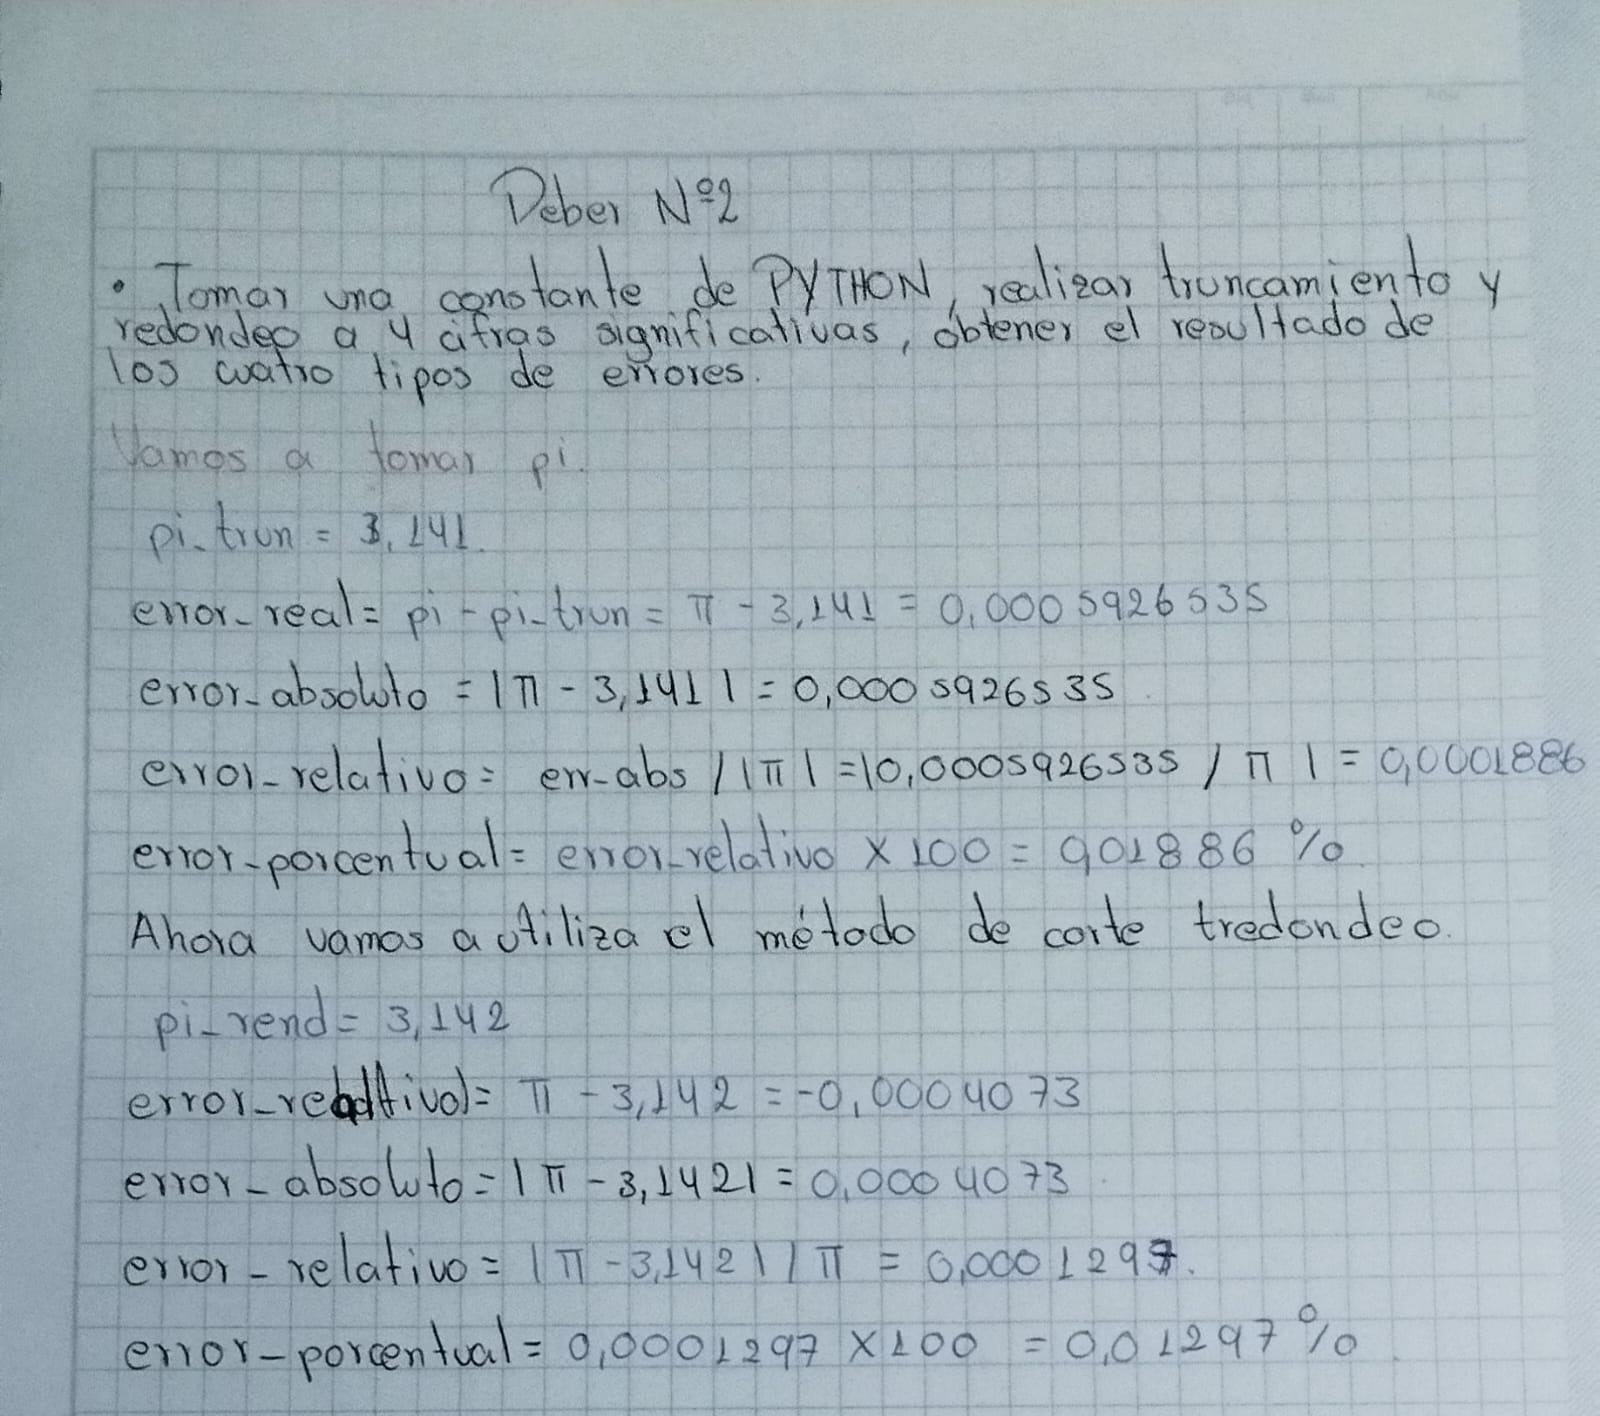
\includegraphics[width=0.50\textwidth]{inFiles/Figures/ConstanteError.jpg}

\vspace{0.25cm}

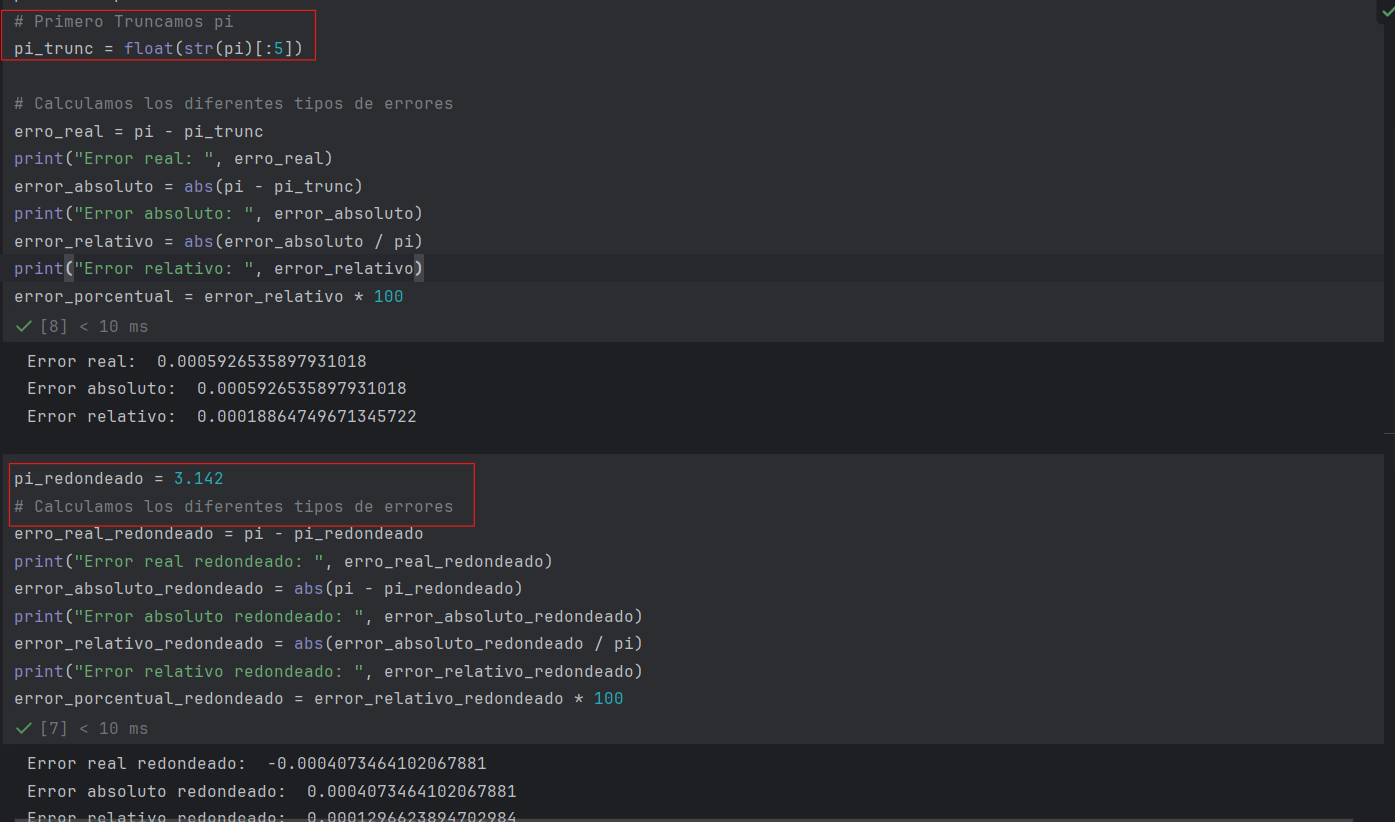
\includegraphics[width=0.98\textwidth]{inFiles/Figures/PythonError.png}

\vspace{0.5cm}
\section*{CONCLUSIONES}
     Dependiendo el metodo de corte que utilicemos vamos a tener una respuesta o otra tanto el metodo de truncamiento
    como el metodo de redondeo son metodos que podemos utilizar sin ningun tipo de problemas, sin embargo en este ejemplo
    si queremos exactitud debemos utilizar el metodo de truncamiento
\end{document}